\chapter{Practical Applications: Training on a Specific Task}

\section{Datasets}

% In the last few years, the most popular dataset for modern object detectors was the Common Objects in Context (COCO) dataset~\footnote{\url{}} \textbf{(source? + insert paper citation)}. The publications discussed in the previous chapters have all been evaluated on the COCO~2017 dataset. It is also used for segmentation, but the object detection dataset in itself contains annotations of 80 classes, so the best models learn fairly general representations of many visual features from objects.

The Microsoft COCO: Common Objects in Context is an immensely popular dataset for numerous computer vision tasks (classification, object detection, instance segmentation, collectively called object recognition). It was introduced in 2014 in the paper \textit{Microsoft COCO: Common Objects in Context} \cite{Coco}, aiming to improve upon already existent visual datasets like ImageNet and PASCAL, and striving to be a benchmark of scene understanding. It contains labeled data for 91 object classes, captured in their natural habitat (hence \textit{context}). It was later updated in 2017, a notable change being the introduction of \textit{stuff} labels (among the already existent \textit{thing} labels), for objects with no clear boundaries, like sky and grass. These wer introduced as panoptic segmentation labels.

The official site of the dataset\footnote{\url{https://cocodataset.org}} mentions that the creators of COCO have partnered with the developers of open source tool FiftyOne in providing a software to facilitate downloading, visualizing, and evaluation on COCO, so I will be using it for intial data exploration. Another tool endorsed by the creators is the COCO API.

% However, in this work I am going to specialise my models of choice for vehicle detection. Theoretically, taking the COCO dataset and stripping all but 2 of its classes, the \textit{car} and \textit{truck} classes provides a vehicular dataset, and eventually chosing images that contain none of the above as \textit{hard negatives} should work satisfactory. However, during the research I have found two vehicle-centered, public datasets available: the kitti dataset, and the UA-DETRAC dataset.

I conducted initial data exploration on the COCO dataset with the FiftyOne tool (launching an application session from a Python shell as described in their tutorials), as seen in figure~\ref{fig:fiftyone-car-truck}. The success of the COCO dataset lies in its richness and difficulty: some training images, as seen in figure \ref{fig:coco-difficult}, are caught in so called \textit{non-iconic views}, where visual features can be ambiguous and they should be interpreted in context to recognise the object.

% \begin{center}
%     \captionof{figure}{Exploring the train split of the MS COCO 2017 dataset in the FiftyOne tool. There are 43867 instances of labeled cars and 9973 instances of labeled trucks, with 14714 images containing either of them.}
%     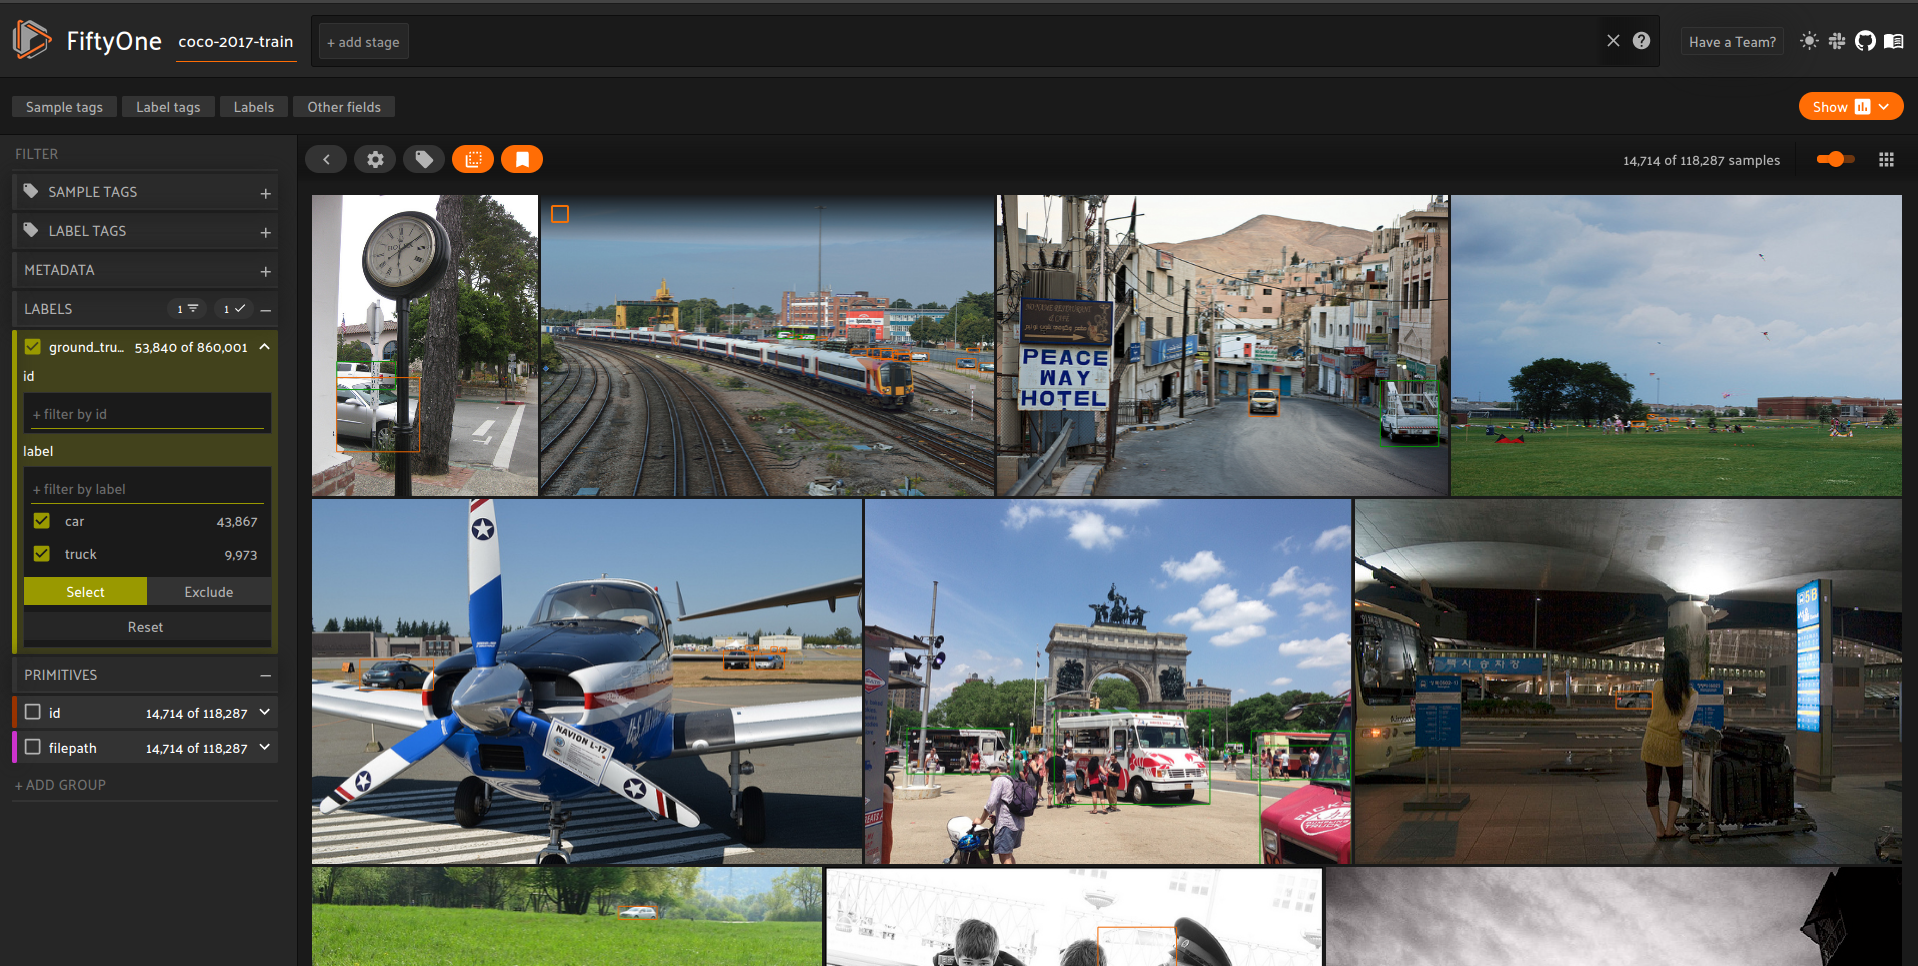
\includegraphics[width=\textwidth]{figures/fiftyone-coco-car-truck.png}
%     \label{fig:fiftyone-car-truck}
% \end{center}

\begin{figure}[h]
    \captionsetup{width=\textwidth}
    \caption{Exploring the train split of the MS COCO 2017 dataset in the FiftyOne tool. There are 43867 instances of labeled cars and 9973 instances of labeled trucks, with 14714 images containing either of them.}
    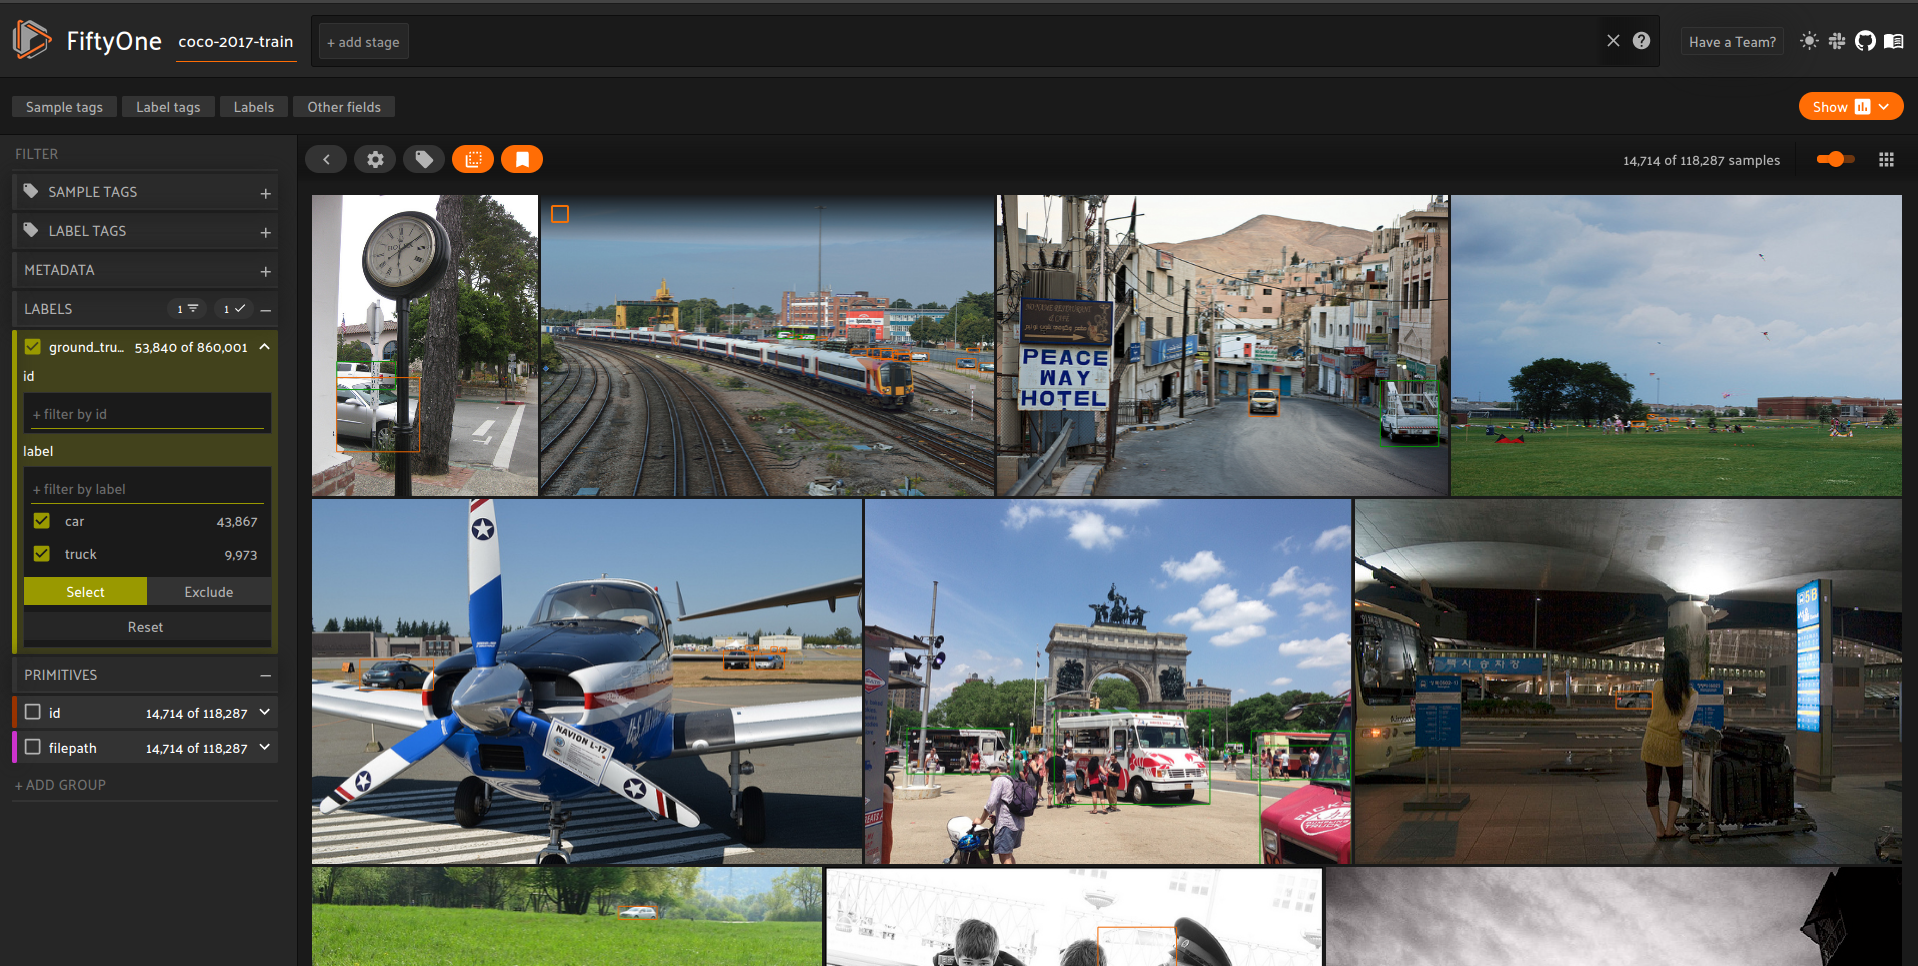
\includegraphics[width=\textwidth]{figures/fiftyone-coco-car-truck.png}\label{fig:fiftyone-car-truck}
\end{figure}

\begin{figure}[h]
    \captionsetup{width=\textwidth}
    \caption{Some difficult examples: objects in overexposed regions of the image, crowd labels consising of very small (e.g aerial) images of cars (orange) and trucks(green), detection based on a skewed reflection of the onject, small parts of it.}
    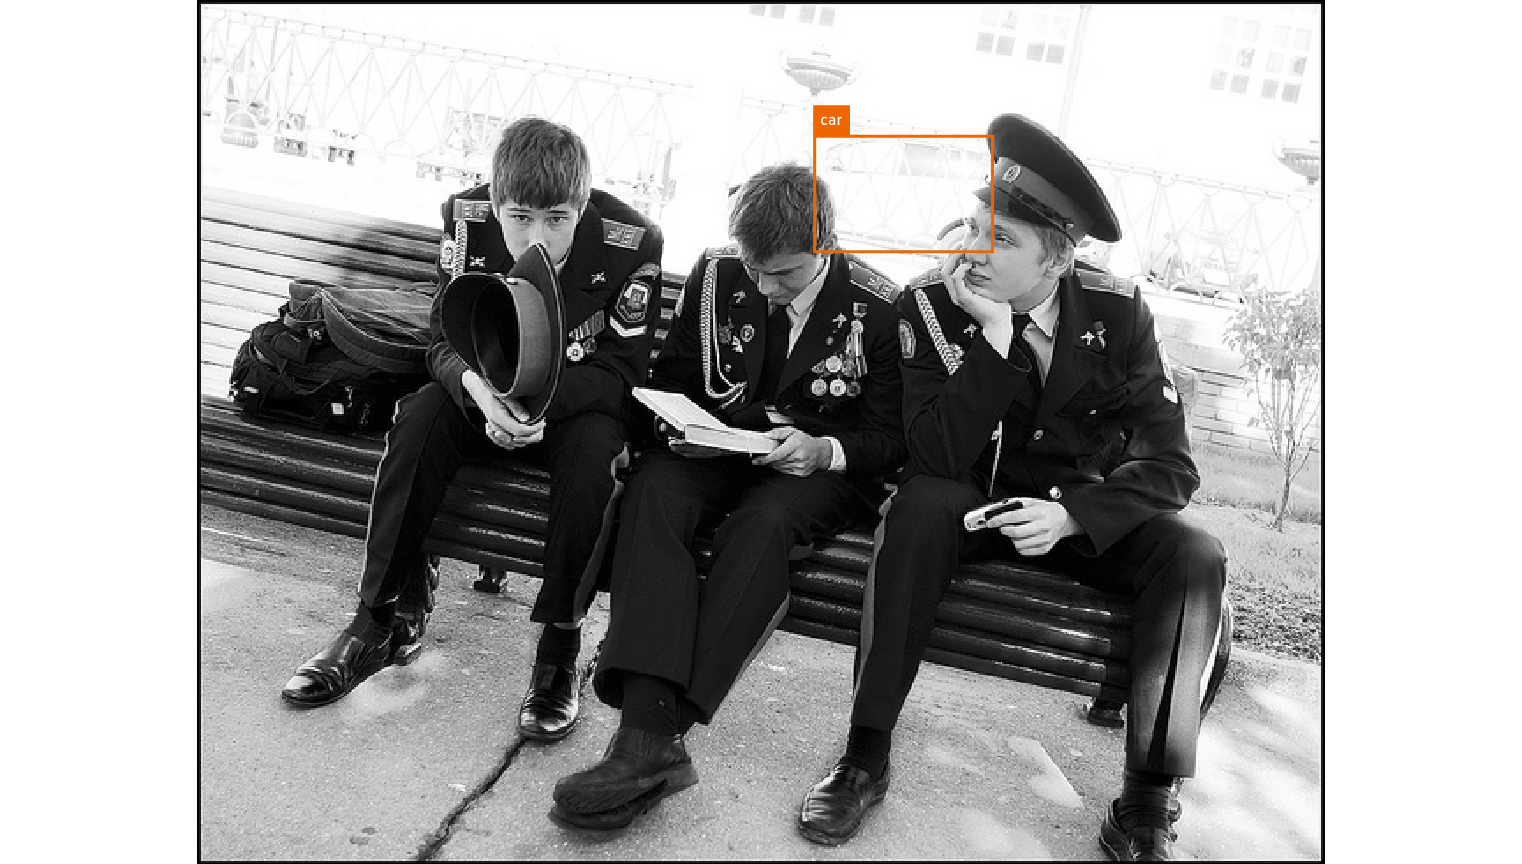
\includegraphics[width=.49\textwidth]{figures/car-overexposed.png}
    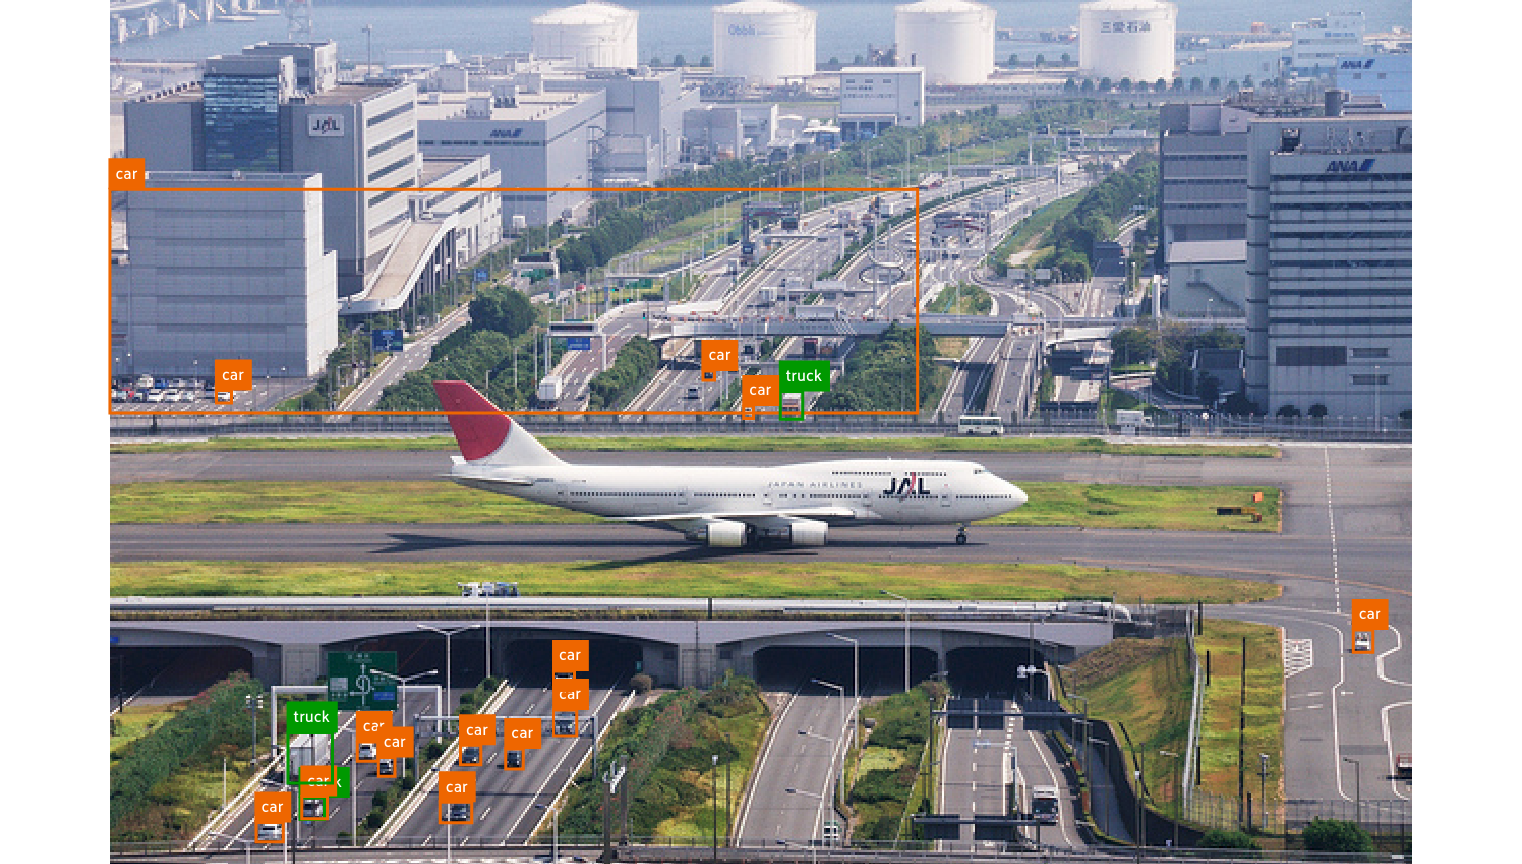
\includegraphics[width=.49\textwidth]{figures/car-truck-small-crowd.png}\\
    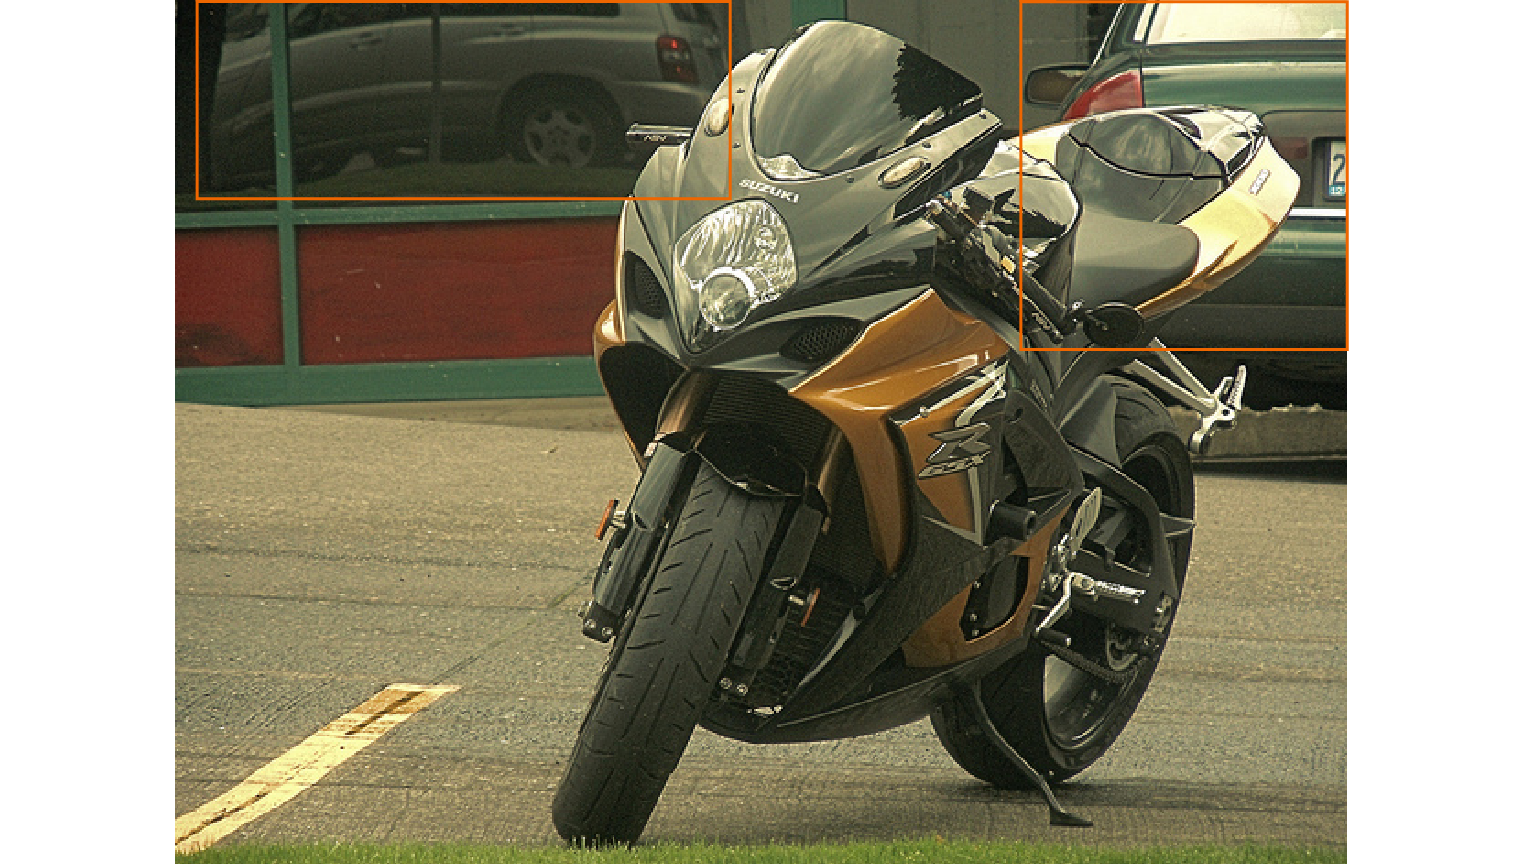
\includegraphics[width=.49\textwidth]{figures/car-reflection-partial.png}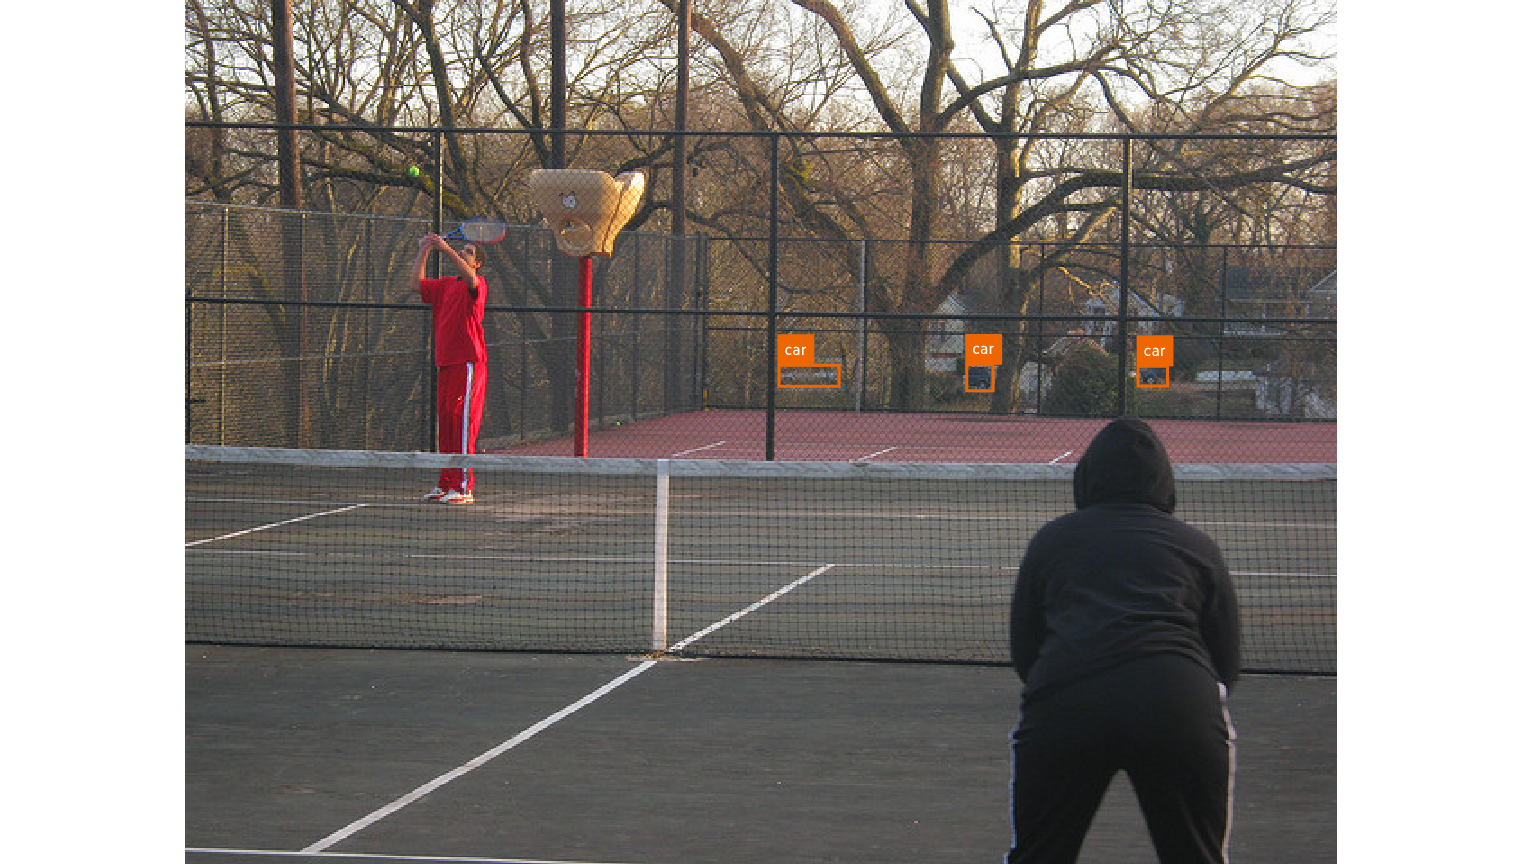
\includegraphics[width=.49\textwidth]{figures/car-obscure.png}\\
    \label{fig:coco-difficult}
\end{figure}

\subsection{Preparing the filtered COCO dataset}


% \subsection{kitti}




% \section{Training via Transfer Learning}

% \subsection{DETR}
